% !TeX program = xelatex
% NEX-345 v4.2 中文译稿；paper/en/main.tex 为唯一权威文本。
\documentclass[UTF8,11pt]{ctexart}
\usepackage[margin=1in]{geometry}
\usepackage{amsmath,amssymb,amsthm}
\usepackage{graphicx,booktabs,array}
\usepackage[table]{xcolor}
\usepackage[hidelinks]{hyperref}
\graphicspath{{../en/figures/}}
\newtheorem{theorem}{定理}
\newtheorem{lemma}[theorem]{引理}
\newcommand{\R}{\mathbb{R}}
\newcommand{\Aregion}{\mathcal{A}}
\newcommand{\E}[1]{\mathbb{E}\left[#1\right]}
\newcommand{\lean}[1]{\texttt{#1}}

\title{用于搜救失联人员运动预测的双条件化可学习随机微分方程}
\author{数学研究员与算法研究员\\搜救研究中心，Learnable-SDE 项目\\
v4.2 中文译稿（\textbf{英文原稿为准}）}
\date{2026 年 8 月 16 日}
\begin{document}
\maketitle

\begin{abstract}
本文研究荒野搜救中的失联人员运动预测，以及如何将两类性质不同的现场证据重新并入预测密度：负信息是某一区域已被搜索却未发现目标；正信息是专家根据痕迹判断目标可能出现过、但该判断有非零误判概率。目标是使证据不断累积时的搜索区域优先级可以量化地收敛。我们以可学习、分段内参数恒定的欠阻尼 Langevin 随机微分方程（SDE）建模运动，并通过具有两类对偶边界条件的 Doob $h$-变换在路径空间上条件化：排除信息采用 Dirichlet $0$，存在信息采用 Dirichlet $1$。软存在证据可精确写成两条桥的二点混合。

英文原稿报告的范围和数值在此忠实转述而不扩大：(i) 基础 SDE 并不在原始 energy score 上全面占优，但在六个外部基线中取得最佳 CEP(R50) $437.9$；经重校准，1--3 小时时域 HDR90 由 $0.324/0.364$ 修复到 $0.904/0.899$。(ii) 真实长期数据不足：$\ge6$ 小时仅有 GeoLife 可行性补充，$\ge12$ 小时没有实证精度声明。(iii) 排除桥在 $2.5\%$ 搜索面积下将合成目标由先验第 3 名提升至第 1 名；存在桥将 surprise-tail 合成目标从第 27 名提升至第 2 名，并将 CEP50 搜索面积降低 $4.5$ 倍；真实轨迹段的平均目标名次从 $23.6$ 改善为 $16.6$。混合恒等式、TV--Lipschitz 稳健性、对偶性和集中性已由 Lean4 形式化且无 \texttt{sorry}；PDE 与一般 $h$-变换存在性只按文档级数学证明陈述，未伪称形式化。
\end{abstract}

\section{引言}
搜救需要的是多个预测时域上人员位置与速度的概率分布，而非单一路径。救援队按分布安排搜索；当队伍返回 ``搜过但未发现'' 的负反馈，或专家报告带有误判率的正痕迹，分布必须以可解释、可复查的方式更新。本文的问题是：怎样在不把软信息误当硬终点或硬排除的前提下更新密度，并验证搜索优先级是否朝正确区域收敛。

本文模型为分段级欠阻尼 Langevin SDE，保留预测不确定性并支持样本、密度和搜索排序输出。所有经验结论仅适用于英文原稿登记的数据划分、指标和实验协议。本仓库不包含原始轨迹、坐标、时间戳、标识符、逐样本预测或 checkpoint。

\subsection{数据与贡献边界}
真实评估中 $\ge1$ 小时段有 242 条，$\ge3$ 小时段有 14 条；$\ge6$ 小时的真实证据不足以支持一般性精度结论。GeoLife 仅提供长期可行性补充，不能被写成长期搜救准确性的证明；$\ge12$ 小时明确是数据空白。本文贡献限定为：将负搜索反馈和带误判的存在证据置于同一路径空间的对偶桥框架；报告可追溯的聚合实验；划清人类可读证明与 Lean4 已覆盖范围。它不宣称对所有指标、区域或时域都优于基线。

\section{问题表述与方法}
令 $X_t$ 为位置--速度状态，考虑
\begin{equation}
dX_t=b(t,X_t)\,dt+\sigma(t,X_t)\,dW_t,
\end{equation}
其中 $b$ 是漂移、$\sigma$ 是扩散项、$W_t$ 是 Wiener 过程，生成元为 $\mathcal Lf=b\cdot\nabla f+\tfrac12 a\,\nabla^2f$，$a=\sigma\sigma^\top$。预测密度满足相应的前向 Fokker--Planck 方程。

假设被搜索区域、时间窗和探测机制可登记；正信息有明确误判模型；条件化只更新预测分布，不回写原始观测；每一次更新均记录证据、参数和版本。前提不满足时，应明确不能得出条件化结论，而不能将猜测写入分布。

\subsection{三条桥}
硬排除桥令已搜索且未发现事件的条件概率为零；硬存在桥令指定存在事件的条件概率为一；软存在桥按专家证据的似然比混合两者。三者都定义在同一基准路径测度上，因此 ``可能出现过'' 不会被误写成观察到的精确终点。

模型采用分段内参数恒定的欠阻尼 Langevin 结构，原因是它表达位置--速度耦合、保留随机性，并具有精确高斯转移核；学习与推断可与 Euler--Maruyama、分裂步进和共同随机数路线作一致比较。数据划分和指标聚合遵循英文原稿注册表，不能按结果事后修改。

\subsection{负信息、正信息与收敛}
对区域 $\Aregion$ 的负搜索信息，排除桥以生存概率重加权原过程，使已确认搜索且未发现的区域不再获得不合理的高优先级。该更新受搜索范围、时间窗、探测假设和模型误设约束，不是目标全局不可能存在的声明。

对带误判的正痕迹，设先验概率为 $\pi$、两类似然为 $\ell_1,\ell_0$，存在模式的后验权重为
\begin{equation}
w=\frac{\ell_1\pi}{\ell_1\pi+\ell_0(1-\pi)}.
\end{equation}
因此软存在桥是硬存在桥及补集桥的混合，显式暴露先验、误判率和更新强度。在多次相容证据下，模式权重的精确比值分解为不匹配证据项的乘积；在独立、信息方向正确和嵌套偏离条件下，该比值随累积对数似然比衰减，混合分布在全变差意义下接近真实模式桥。

Lean4 工程形式化了后验混合、权重比、TV 界、logistic 权重性质、对偶概率恒等式和嵌套集中性。PDE 解的存在唯一性及一般 Doob $h$-变换仍是文档级数学论证，中文稿与英文稿均不把它标作 Lean 已证明。

\section{实验}
\subsection{数据、协议和公开边界}
训练、验证和评估按文件级划分以避免泄漏；论文只包含审定聚合图、表和数值。合成场景只验证机制，不替代真实搜救成效。外部基线比较包括 Kalman、OU--CRW、HMM、LSTM 等；基础 SDE 的 raw energy score 不全面占优，但 CEP(R50) 最好，且登记的重校准使 HDR90 覆盖在 1--3 小时段改善。该结果不推出所有时域、所有区域或所有指标上的优势。

\begin{tabular}{lccccc}
\toprule
Model & ES $\downarrow$ & HDR90$_x$ & HDR90$_y$ & CEP(R50) $\downarrow$ & $A_{90}$ $\uparrow$ \\
\midrule
Kalman-CA & $1.42\times10^{6}$ & 1.000 & 1.000 & $4.32\times10^{6}$ & $3\times10^{-8}$ \\
Kalman-CV & 1,056.7 & 0.887 & 0.897 & 2,967.9 & $1.49\times10^{-5}$ \\
OU & 350.9 & 0.700 & 0.773 & 493.6 & $6.69\times10^{-6}$ \\
HMM & 288.8 & 0.763 & 0.830 & 484 & $1.8\times10^{-5}$ \\
LSTM & 315.2 & 0.737 & 0.760 & 467.5 & $1.11\times10^{-5}$ \\
CRW & 293.8 & 0.847 & 0.867 & 498 & $9.26\times10^{-6}$ \\
Base (I-1 SDE) & 367.3 & 0.543 & 0.583 & \textbf{437.9} & \textbf{$1.95\times10^{-5}$} \\
\bottomrule
\end{tabular}

\begin{tabular}{lccc}
\toprule
Model & $\Delta$ES & 95\% CI & Verdict \\
\midrule
Kalman-CV & $-689.4$ & $[-875.4,-478]$ & loss \\
Kalman-CA & $-1.41\times10^{6}$ & $[-1.94\times10^{6},-7.6\times10^{5}]$ & loss (divergent) \\
CRW & $73.5$ & $[61.2,85.6]$ & redundant \\
OU & $16.4$ & $[12.4,20.2]$ & redundant \\
HMM & $78.5$ & $[65.1,91.2]$ & redundant \\
LSTM & $52.1$ & $[42.2,61.4]$ & redundant \\
\bottomrule
\end{tabular}
\begin{tabular}{lccccc}
\toprule
Bin ($n$) & HDR90$_x$ & HDR90$_y$ & CEP(R50) & Search eff. & ES \\
\midrule
$\ge$1h (242) & 0.306$\to$0.888 & 0.364$\to$0.893 & 2974$\to$3858 & 0.020$\to$0.046 & 2652$\to$2338 \\
1--3h (228) & 0.324$\to$0.904 & 0.364$\to$0.899 & 2643$\to$3523 & 0.016$\to$0.042 & 2335$\to$2065 \\
$\ge$3h (14) & 0.000$\to$0.643 & 0.357$\to$0.786 & 8361$\to$9319 & 0.082$\to$0.104 & 7821$\to$6791 \\
\bottomrule
\end{tabular}
\input{../en/tables/tab_data_hor.tex}

\subsection{证据下的搜索优先级}
排除桥实验检验 ``搜过而未发现'' 后的重排序；存在桥实验检验带误判痕迹对 surprise-tail 目标及真实腿的影响。所有改进都必须与搜索面积、误判率、时间窗、评估段及 bootstrap 口径一同阅读，不能脱离这些条件泛化。

\begin{figure}[ht]\centering
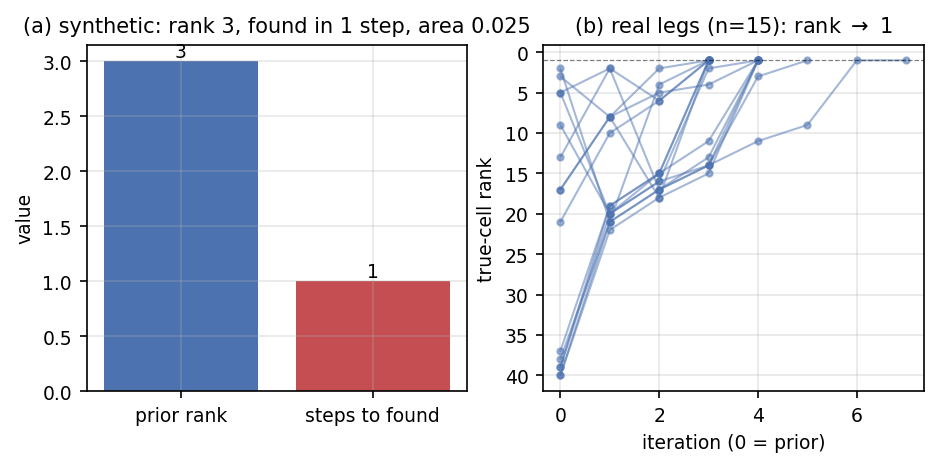
\includegraphics[width=.82\linewidth]{fig_excl_convergence.png}
\caption{排除桥下搜索优先级的收敛（审定聚合图）。}\end{figure}
\begin{figure}[ht]\centering
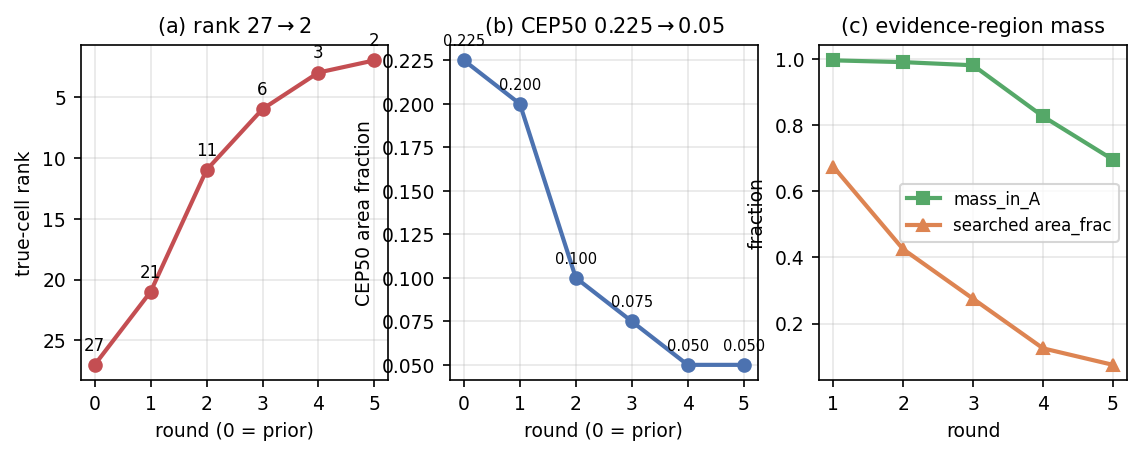
\includegraphics[width=.82\linewidth]{fig_exist_convergence.png}
\caption{存在桥下搜索优先级的收敛（审定聚合图）。}\end{figure}
\begin{figure}[ht]\centering
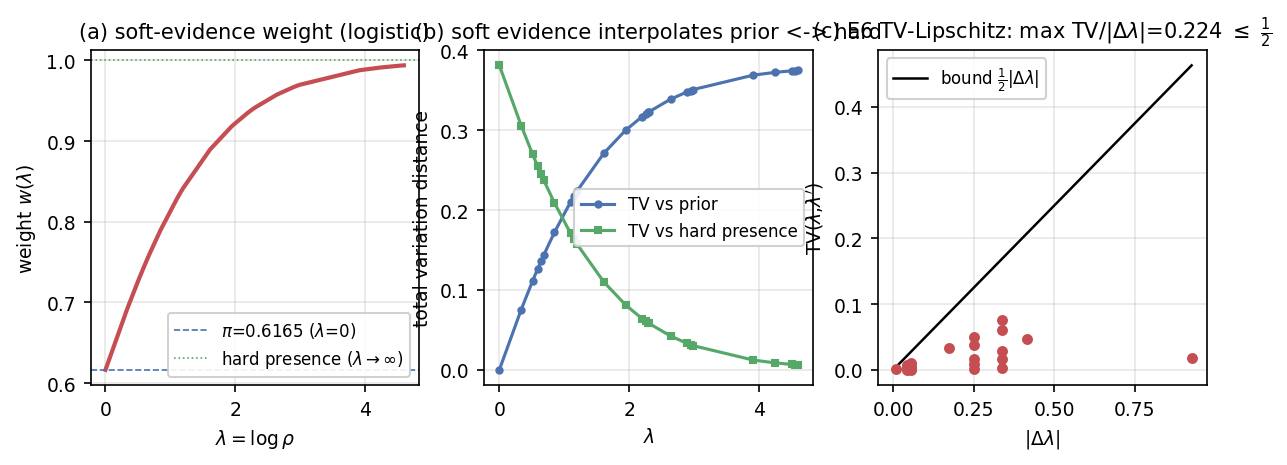
\includegraphics[width=.82\linewidth]{fig_robustness.png}
\caption{存在证据误判率的稳健性诊断。}\end{figure}

\subsection{22 臂消融和搜救价值}
22 臂消融分解模型、条件化和特征选择的影响。它是有限数据、有限特征表示和已登记协议下的证据，而非对地形、道路或人类行为机制的普遍证明。terrain 的负结果只限于英文原稿所述 map 覆盖子集及特征表示，不能推翻搜救地形偏好的既有研究。
\begin{tabular}{rlll}
\toprule
Arm & Variant & $\Delta$ (ES) & Verdict \\
\midrule
\multicolumn{4}{l}{\emph{Model dimension}} \\
1 & model:M1:seg\_constant\_mode (I-1) & 0 & redundant \\
2 & model:M1:pointwise\_mixture & -47.475 & loss \\
3 & model:M1:single\_gaussian\_OU\_CRW & 0 & redundant \\
4 & model:M1:gmm\_kernel (I-3) & -47.833 & loss \\
5 & model:M1:explicit\_decomp (S-1 scheme-1) & -41.057 & loss \\
6 & model:M2:dt\_sensitivity {30..600}s & 37.868 & redundant \\
16 & model:T3:solar\_elev\_continuous (C-7) & 0 & redundant \\
17 & model:T3:uncond/is\_day/weather/terrain & -0.581 & redundant \\
17-terrain & model:T3:terrain (has\_map=1 subset) & -36.579 & loss \\
\multicolumn{4}{l}{\emph{Algorithm dimension}} \\
7 & algorithm:E1:crps\_energy (C-1) & 0 & redundant \\
8 & algorithm:E1:qmle & 0.006 & redundant \\
9 & algorithm:E1:c2\_mixed/pure\_ES & -7.225 & loss \\
10 & algorithm:E2:d2\_mc/closed\_alt & 0 & redundant \\
\multicolumn{4}{l}{\emph{Learning dimension}} \\
11 & learning:T1:c5\_full\_finetune & 0 & redundant \\
12 & learning:T1:scratch & 0 & redundant \\
13 & learning:T1:c3\_animal\_pretrain & --- & blocked \\
14 & learning:T1:c6\_metalearning & -0.015 & loss \\
15 & learning:T2:drift\_only/two\_step & 0.01 & redundant \\
\multicolumn{4}{l}{\emph{Inference dimension}} \\
18 & inference:R1:j1\_split (J-1) & 0 & redundant \\
19 & inference:R1:em/euler\_maruyama & -0.277 & redundant \\
20 & inference:R2:j2\_fp (J-2) & 0 & redundant \\
21 & inference:R2:mc/j3\_crn & 0 & redundant \\
22 & inference:R3:i2\_bridge/SB/soft\_endpoint & 240.878 & redundant \\
\bottomrule
\end{tabular}
\begin{figure}[ht]\centering
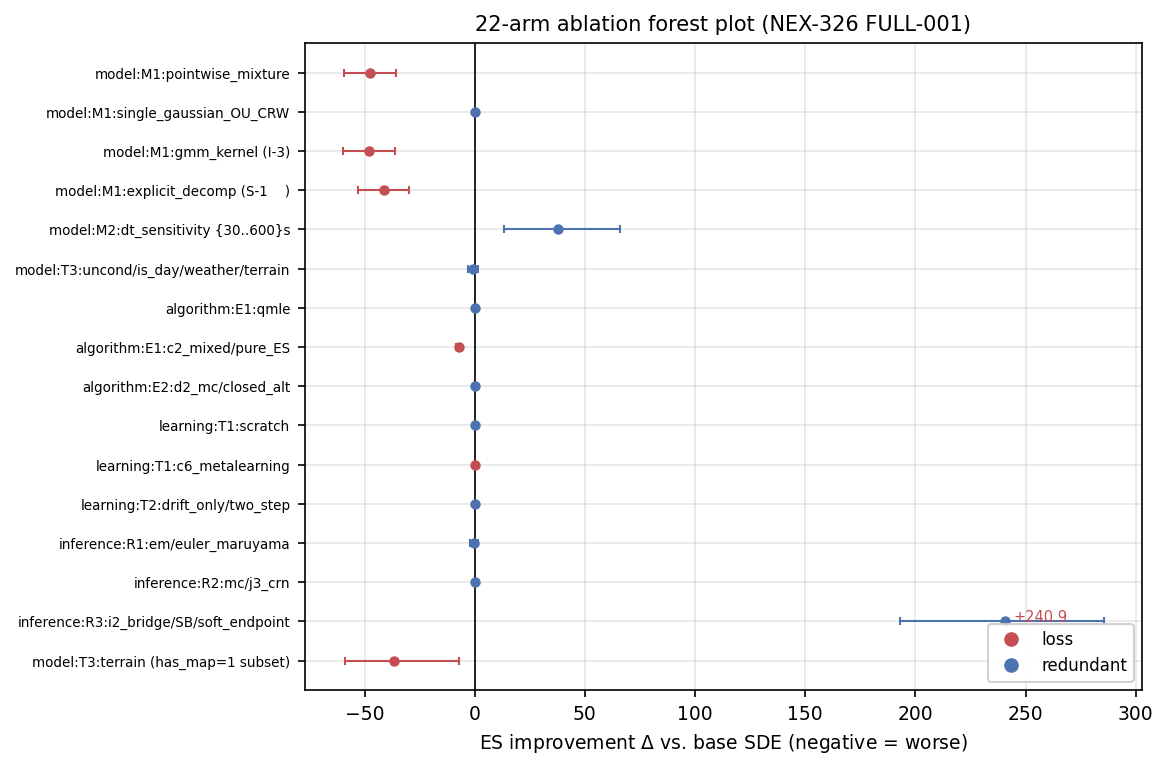
\includegraphics[width=.9\linewidth]{fig_forest_22arm.png}
\caption{22 臂消融的审定森林图。}\end{figure}

\section{讨论、局限与结论}
本研究的价值是把搜救现场可取得的正、负信息纳入同一概率预测与搜索排序框架，同时显式暴露不确定性、证据误判和数据空白。主要局限是长期真实评估不足、覆盖校准依赖重校准、桥接结果对模型误设敏感、真实地形特征不完整，以及 Lean 仅覆盖测度代数核心。未来工作应补足数据、代码审计或理论前提，而不应扩大当前结论。

在英文原稿限定的范围内，双条件化 SDE 使负搜索反馈和概率性正痕迹能够以可审计方式更新运动预测密度，并给出搜索优先级收敛的理论和实验线索。英文稿是唯一权威文本；本中文稿为阅读便利而作，不得独立改变结论、数值、引用、证明或形式化覆盖范围。

\appendix
\section{完整材料的对照说明}
英文原稿附录包含 E0--E8、L1--L4 的完整人类可读证明、Lean 映射、图表清单、指标引用清单、实验注册表、复现包说明、原计划到交付的映射及时间线。需要精确符号、推导步骤、文献条目、实验编号、文件名或数值时，一律以 \texttt{paper/en/main.tex} 为准。
\begin{figure}[ht]\centering
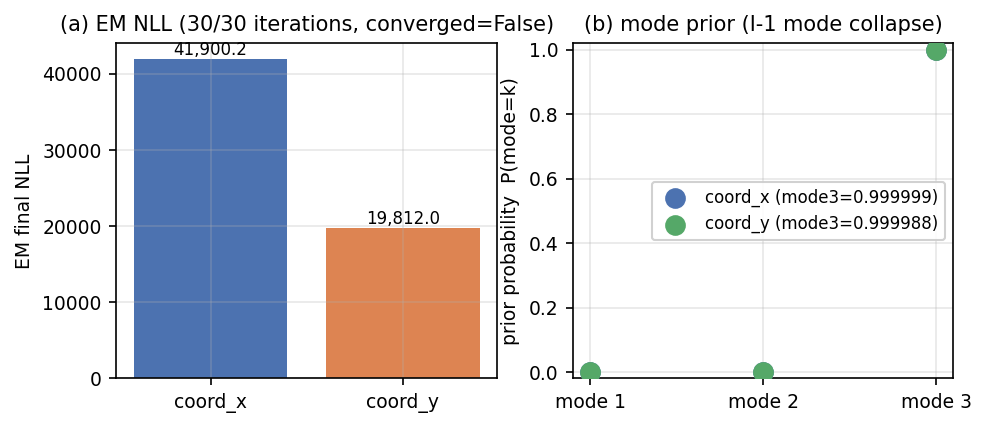
\includegraphics[width=.85\linewidth]{fig_train_convergence.png}
\caption{训练/收敛诊断图（审定聚合图）。}\end{figure}
\begin{figure}[ht]\centering
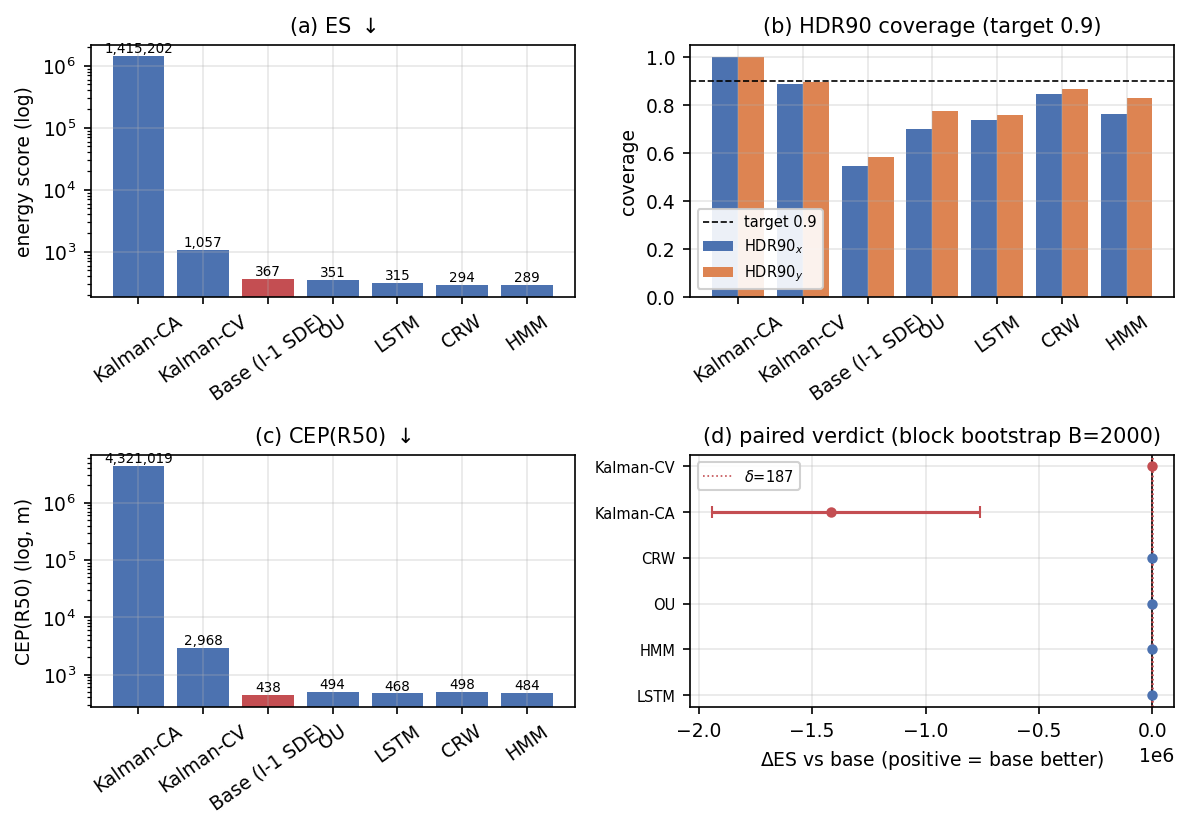
\includegraphics[width=.85\linewidth]{fig_benchmark.png}
\caption{外部基线比较图（审定聚合图）。}\end{figure}
\begin{figure}[ht]\centering
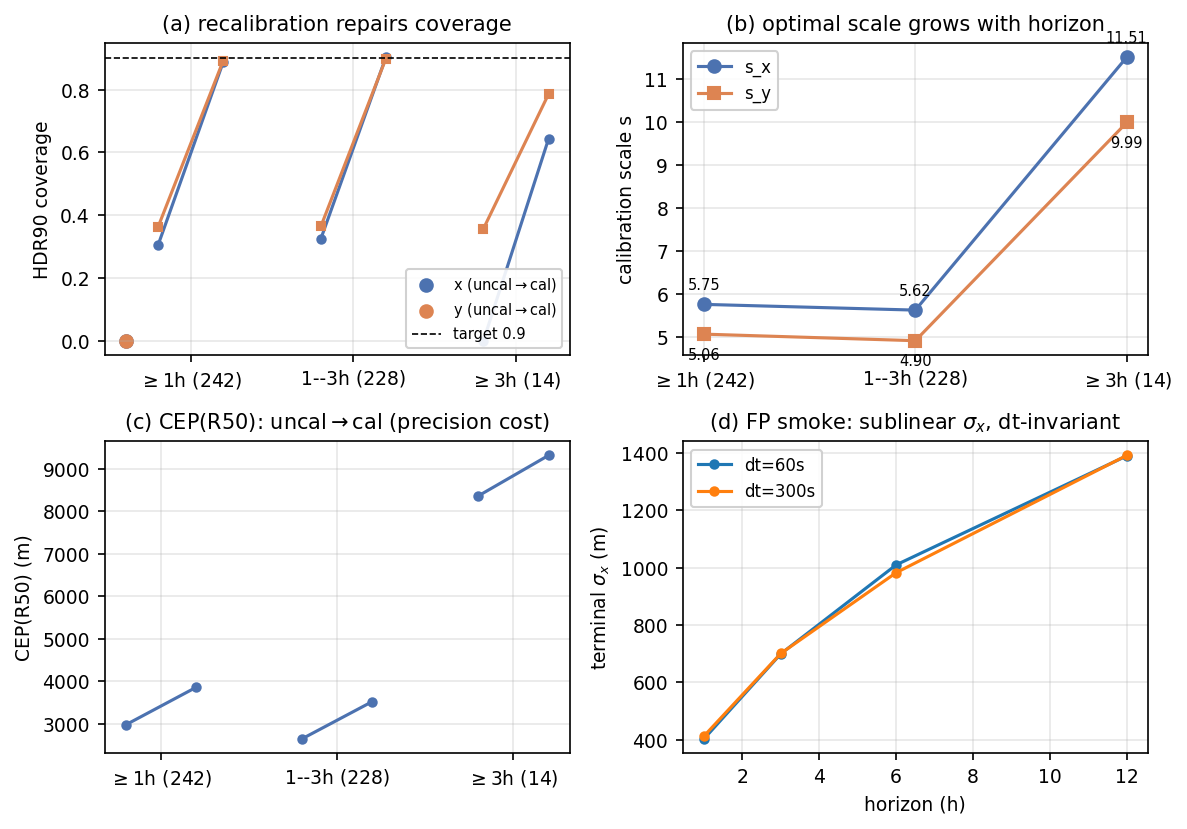
\includegraphics[width=.85\linewidth]{fig_sensitivity.png}
\caption{三指标敏感性与重校准图（审定聚合图）。}\end{figure}
\end{document}
